\documentclass{article}

\usepackage{alltt}
\renewcommand{\ttdefault}{txtt}

\usepackage{graphicx}
\newcommand{\HRule}{\rule{\linewidth}{0.5mm}}

\usepackage{soul}
\usepackage{color}

\sethlcolor{yellow}

\usepackage{listings}

\usepackage{color}
\definecolor{lightgray}{rgb}{.9,.9,.9}
\definecolor{darkgray}{rgb}{.4,.4,.4}
\definecolor{purple}{rgb}{0.65, 0.12, 0.82}

\lstdefinelanguage{JavaScript}{
  keywords={typeof, new, true, false, catch, function, return, null, catch, switch, var, if, in, while, do, else, case, break},
  keywordstyle=\color{blue}\bfseries,
  ndkeywords={class, export, boolean, throw, implements, import, this},
  ndkeywordstyle=\color{darkgray}\bfseries,
  identifierstyle=\color{black},
  sensitive=false,
  comment=[l]{//},
  morecomment=[s]{/*}{*/},
  commentstyle=\color{purple}\ttfamily,
  stringstyle=\color{red}\ttfamily,
  morestring=[b]',
  morestring=[b]"
}

\lstset{ %
  language=JavaScript,
  extendedchars=true,
  basicstyle=\footnotesize\ttfamily,
  showstringspaces=false,
  showspaces=false,
  numbers=left,
  numberstyle=\footnotesize,
  numbersep=9pt,
  tabsize=2,
  breaklines=true,
  showtabs=false,
  captionpos=b
}

\let\oldsection\section 
\renewcommand{\section}{\clearpage\oldsection} 

\begin{document}

\begin{titlepage}

\begin{center}


% Upper part of the page

\includegraphics[width=0.20\textwidth]{./sjsu.jpg}\\[1cm]    

\textsc{\LARGE San Jose State University}\\[1.5cm]

\textsc{\Large Network \& Protocols Project 2}\\[0.5cm]


% Title
\HRule \\[0.6cm]
{ \huge \bfseries Simulation of Ethernet Medium Access Control protocols}\\[0.4cm]

\HRule \\[1.5cm]

% Author and supervisor
\begin{center}
Alexandre \textsc{Joseph} \\
Audric \textsc{Albaret} \\
Nicolas \textsc{Roux} 
\end{center}
\vfill

% Bottom of the page
{\large \today}

\end{center}

\end{titlepage}


\setcounter{tocdepth}{2}

\tableofcontents

\clearpage

% \section{Proposal}



\subsection{Description}

\begin{description}
    \item Protocol : Ethernet
    \item MAC protocol : CSMA / CD
    \item Computer language : JavaScript, HTML5
    \item Platform : ALL
\end{description}

\subsection{The high-level description of the simulation algorithm}


\begin{center}
\item Algorithm for CSMA /CD
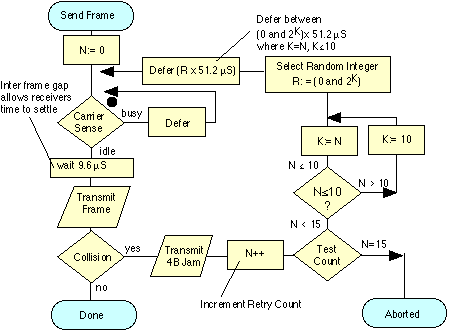
\includegraphics[scale=0.8]{ether.png}
\end{center}

\newpage

\subsection{The mathematical formulae}

\subsubsection{Synchronous data traffic}
Packet arrival and inter arrival time are all uniform and deterministic.
\begin{description}
    \item Arrival process : packet size / bandwidth ( packets/sec)
    \item Traffic load = packet arrival time rate * packet size
    \item Average packet delay = transmission time for one packet
    \item Delay Variance = 0 because intervals are equal.
    \item Thoughput = $\frac{number of byte sent}{total time}$
\end{description}

\subsubsection{Asynchronous data traffic}

\begin{description}
    \item Arrival process : $ \frac{e^{b} \cdot b^{k}}{k!}$ (Poisson distribution)
    \item Traffic load = packet arrival time rate  (Poisson distribution : $ \frac{e^{b} \cdot b^{k}}{k!}$) $\times$ packet size (Exponential distribution : $\lambda \cdot e^{ \lambda \cdot t}$)
	\begin{description}  
    \item b = $\lambda \cdot$t
    \item t is used to define the interval 0 to t   
    \item $\lambda$ is the total average arrival rate in packets
   	\item k is the total number of packets in the interval 0 to t
   	\end{description}
    \item Average packet delay = $\overline{x} = \dfrac{1}{n} \sum_{i=1}^{n} x_{i}$
    \item Delay Variance = $ V(X) = \dfrac{1}{n} \sum_{i=1}^{n} x_{i}^{2} - \overline{x}$
    	\begin{description}
    	\item X : Delay
    	\item n = number of packets
    	\item $x_{i}$ = delay for packet number \begin{tiny}
•
\end{tiny}i
    	\item $\overline{x}$ = average packet delay
       	\end{description}
    \item Thoughput = $\frac{number of byte sent}{total time}$
\end{description}

\subsection{The list of references}
\begin{description}
\item Chapter 2 of the textbook by Peterson and Davie
\item The set of handout on simulation provided.
\item \href{http://mathworld.wolfram.com/PoissonDistribution.html}{http://mathworld.wolfram.com/PoissonDistribution.html}
\item \href{http://www.erg.abdn.ac.uk/~gorry/eg3561/lan-pages/csma-cd.html}{http://www.erg.abdn.ac.uk/~gorry/eg3561/lan-pages/csma-cd.html}
\end{description}


\section{Proposal}



\subsection{Description}

\begin{description}
    \item Protocol : Ethernet
    \item MAC protocol : CSMA / CD
    \item Computer language : JavaScript, HTML5
    \item Platform : ALL
\end{description}

\subsection{The high-level description of the simulation algorithm}


\begin{center}
\item Algorithm for CSMA /CD
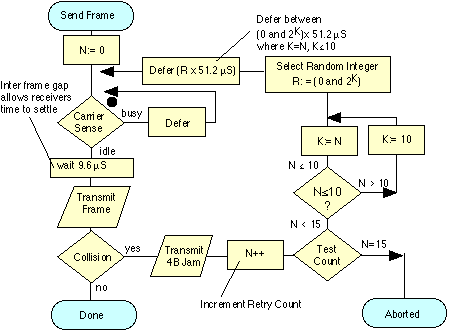
\includegraphics[scale=0.8]{ether.png}
\end{center}

\newpage

\subsection{The mathematical formulae}

\subsubsection{Synchronous data traffic}
Packet arrival and inter arrival time are all uniform and deterministic.
\begin{description}
    \item Arrival process : packet size / bandwidth ( packets/sec)
    \item Traffic load = packet arrival time rate * packet size
    \item Average packet delay = transmission time for one packet
    \item Delay Variance = 0 because intervals are equal.
    \item Thoughput = $\frac{number of byte sent}{total time}$
\end{description}

\subsubsection{Asynchronous data traffic}

\begin{description}
    \item Arrival process : $ \frac{e^{b} \cdot b^{k}}{k!}$ (Poisson distribution)
    \item Traffic load = packet arrival time rate  (Poisson distribution : $ \frac{e^{b} \cdot b^{k}}{k!}$) $\times$ packet size (Exponential distribution : $\lambda \cdot e^{ \lambda \cdot t}$)
	\begin{description}  
    \item b = $\lambda \cdot$t
    \item t is used to define the interval 0 to t   
    \item $\lambda$ is the total average arrival rate in packets
   	\item k is the total number of packets in the interval 0 to t
   	\end{description}
    \item Average packet delay = $\overline{x} = \dfrac{1}{n} \sum_{i=1}^{n} x_{i}$
    \item Delay Variance = $ V(X) = \dfrac{1}{n} \sum_{i=1}^{n} x_{i}^{2} - \overline{x}$
    	\begin{description}
    	\item X : Delay
    	\item n = number of packets
    	\item $x_{i}$ = delay for packet number \begin{tiny}
•
\end{tiny}i
    	\item $\overline{x}$ = average packet delay
       	\end{description}
    \item Thoughput = $\frac{number of byte sent}{total time}$
\end{description}

\subsection{The list of references}
\begin{description}
\item Chapter 2 of the textbook by Peterson and Davie
\item The set of handout on simulation provided.
\item \href{http://mathworld.wolfram.com/PoissonDistribution.html}{http://mathworld.wolfram.com/PoissonDistribution.html}
\item \href{http://www.erg.abdn.ac.uk/~gorry/eg3561/lan-pages/csma-cd.html}{http://www.erg.abdn.ac.uk/~gorry/eg3561/lan-pages/csma-cd.html}
\end{description}


\section{Print-out some code}

\begin{lstlisting}[caption=My Javascript Example]
/**
 * Paquito network simulation
 * 
 * @version 0.1
 */
var PKT = function () {
	var _frame = FRM;
	var _sender = SDR;
	var _reciever = RCR;
	
	var _settings = {
		debug: true, // output debug info
		debugMode: 'console', // debug output method ('console' or 'alert')
	};
	
	/**
	 * Output Paquito debug information
	 * @param {String} msg Message to print
	 */
	var _debug = function(msg) {
		msg = 'Paquito: ' + msg;
		if(_settings.debug)
		{
			switch(_settings.debugMode) {
				case 'alert':
					alert(msg);
					break;
				case 'console':
					console.log(msg);
					break;
				default:
					alert(msg);
					break;
			}
		}
	};

	var _test = function () {
		_frame.payload('01010101');
		_debug(_frame.crc());
	};
	
	/**
	 * Initialize Paquito
	 * @param {Object} settings
	 */
	var _init = function(settings) {
		for(attr in settings) {
			_settings[attr] = settings[attr];
		}
		
		_debug('Initialized');
		
		_test();
	};
	
	// expose public properties and methods
	return {
		init: _init,
	};
}();
\end{lstlisting}

\subsection{Inserting an image}

\begin{center}
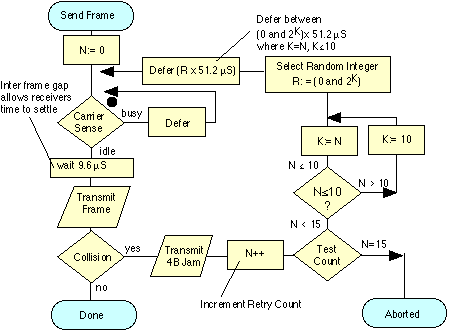
\includegraphics[scale=0.8]{ether.png}
\end{center}



\end{document}
